\documentclass[conference,onecolumn]{IEEEtran}
\IEEEoverridecommandlockouts
% The preceding line is only needed to identify funding in the first footnote. If that is unneeded, please comment it out.
\usepackage{cite}
\usepackage{amsmath,amssymb,amsfonts}
\usepackage{algorithmic}
\usepackage{graphicx,subcaption}
\usepackage{float}
\usepackage{hyperref}
\usepackage{textcomp}
\usepackage{xcolor}
\usepackage{listings}
\usepackage{enumitem}
\usepackage{booktabs}
\usepackage{multirow}
\usepackage{array}
\usepackage{minted}

\DeclareMathOperator*{\argmax}{arg\,max}
\DeclareMathOperator*{\argmin}{arg\,min}

\def\BibTeX{{\rm B\kern-.05em{\sc i\kern-.025em b}\kern-.08em
    T\kern-.1667em\lower.7ex\hbox{E}\kern-.125emX}}

\IEEEoverridecommandlockouts

\lstset{
    language=MATLAB,             % Set language to MATLAB
    basicstyle=\ttfamily\small,  % Set font to small and monospaced
    keywordstyle=\color{blue},   % Color keywords
    stringstyle=\color{orange},   % Color strings
    commentstyle=\color{gray},   % Color comments
    showstringspaces=false,      % Do not display string spaces
    frame=single,                % Add a frame around the code
    breaklines=true              % Line breaks for long lines
}

\setlist[enumerate,1]{label=\arabic{enumi}.}
\setlist[enumerate,2]{label=(\alph*)}
\setlist[enumerate,3]{label=\roman*.}

\begin{document}

\title{\Large Assignment 6 --- Math Fundamentals for Robotics 16-811, Fall 2024}

\author{
      \IEEEauthorblockN{Mukai Yu}
      \IEEEauthorblockA{\textit{MSR, CMU} \\
            Pittsburgh, PA\\
            \href{mailto:mukaiy@andrew.cmu.edu}{mukaiy@andrew.cmu.edu}}
}

\maketitle

\begin{enumerate}
      \item Implement two-dimensional (2D) convex hull.

            Your algorithm should take as input a finite set of 2D points and produce as output a polygon constituting the boundary of the minimal convex set containing all the input points.
            (“minimal convex set” means that the set is a subset of any other convex set that contains all the input points.)

            \textbf{Solution:}

            \begin{lstlisting}[language=Python]
def min_convex_set(points: np.ndarray) -> np.ndarray:
      """
      Compute the convex hull of a set of 2D points using Graham's scan algorithm.

      Args:
            points (np.ndarray): An array of shape (n, 2) containing 2D points.

      Returns:
            np.ndarray: An array of 2D points representing the vertices of the convex hull
                        in counterclockwise order.
      """
      # Input check
      assert points.shape[1] == 2, "Input points should be 2D"
      _points = points.copy().reshape(-1, 2)

      # Step 1: Find the bottom-most point (or the leftmost if there's a tie)
      bottom = _points[np.lexsort((_points[:, 0], _points[:, 1]))[0]]

      # Step 2: Sort the points by polar angle with respect to the bottom point
      def polar_angle(p):
            return np.arctan2(p[1] - bottom[1], p[0] - bottom[0])

      _points = sorted(_points, key=lambda p: (polar_angle(p), np.linalg.norm(p - bottom)))

      # Step 3: Initialize the convex hull with the first two points
      convex_hull = [_points[0], _points[1]]

      # Step 4: Iterate through the points to construct the convex hull
      for point in _points[2:]:
            while len(convex_hull) >= 2:
                  # Check the orientation of the last three points
                  p1, p2 = convex_hull[-2], convex_hull[-1]
                  cross_product = (p2[0] - p1[0]) * (point[1] - p1[1]) - (p2[1] - p1[1]) * (point[0] - p1[0])
                  if cross_product <= 0:  # Remove the last point if it makes a non-left turn
                        convex_hull.pop()
                  else:
                        break
            convex_hull.append(point)

      return np.array(convex_hull)
            \end{lstlisting}

            \begin{figure}[H]
                  \centering
                  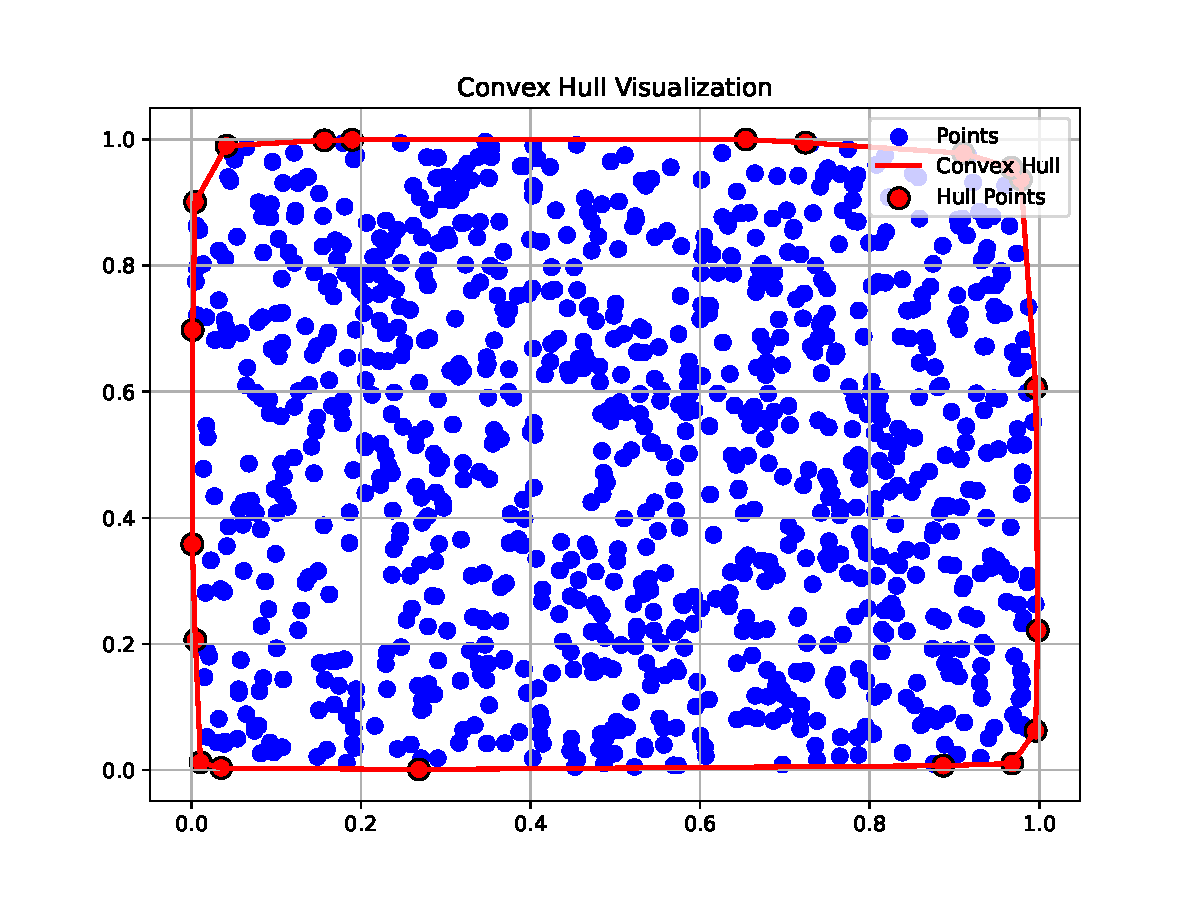
\includegraphics[width=0.99\textwidth]{figs/convex_hull.pdf}
                  \caption{Convex hull of a set of 2D points}
            \end{figure}

            \clearpage
      \item Implement an algorithm for finding shortest paths in 2D polygonal environments.

            The input to your algorithm should consist of a collection of nondegenerate convex polygons, a start location, and a goal location.
            The output should be a piecewise linear path that does not pass through the interior of any polygon and is as short as possible, if such a path exists.
            (Otherwise, your algorithm should indicate that no path exists.)
            One situation in which no path exists is if the start or goal is in the interior of a polygon.

            Notes: (i) The polygons are allowed to overlap.
            (ii) The solution path is allowed to touch the boundaries of polygons, but is not allowed to pass through any polygon's interior.

            \clearpage
      \item Combine your code for parts (1) and (2), along with some additional code, to implement shortest-path motion planning for convex polygons in two dimensions (translations only, no rotations).

            Specifically, the input to your algorithm should consist of a “robot” and its environment, along with start and goal configurations for the robot.
            The output should be a piecewise linear path as described below.
            (The robot moves only in straight lines.
            No rotations.)

            The robot should be a nondegenerate convex polygon.
            The environment should consist of a collection of nondegenerate (possibly overlapping) convex polygons.
            Given start and goal configurations of the robot, your algorithm should produce a shortest intersection-free path between the start and goal, if such a path exists.
            “Intersection-free” means that the robot may touch obstacle boundaries, even slide along obstacle boundaries, but may not touch the interior of any obstacle.
            If no such path exists, your algorithm should report that fact.
\end{enumerate}

\end{document}
